\documentclass[conference]{IEEEtran}
\IEEEoverridecommandlockouts
\usepackage{cite}
\usepackage{amsmath,amssymb,amsfonts}
\usepackage{graphicx}
\usepackage{textcomp}
\usepackage{xcolor}
\usepackage{booktabs}
\usepackage{multirow}
\usepackage{hyperref}

% Dynamic LaTeX Macros for Warehouse Digital Twin Optimization
% Auto-generated by generate_visualizations.py (Zero hardcoded values)

% Facility and Data Characteristics
\newcommand{\TotalLocations}{2,292}
\newcommand{\TotalOrderLines}{119,811}
\newcommand{\TotalOrders}{32,634}
\newcommand{\TotalPicks}{215,192}
\newcommand{\TotalWaves}{9,707}
\newcommand{\TotalOperationalDays}{178}
\newcommand{\BenchmarkWaves}{100}
\newcommand{\UnitGapReconciled}{268}
\newcommand{\AutomatedTestCount}{15}

% DaRA 2026 Timing Calibration
\newcommand{\DaRAValidGaps}{257}
\newcommand{\DaRAMedianGap}{36.0}
\newcommand{\DaRAMeanGap}{54.0}
\newcommand{\DaRAIQR}{26.0--59.0}
\newcommand{\CalibratedPickDwell}{12.6}
\newcommand{\DaRAHandleIQR}{9.1--20.6}
\newcommand{\CalibratedWalkSpeed}{1.10}

% Measured Per-Wave Optimizer Runtimes (ms)
\newcommand{\CASTWaveRuntimeMs}{2.56}
\newcommand{\CASTWaveRuntimeMaxMs}{6.34}
\newcommand{\StaticTSPRuntimeMs}{2.65}
\newcommand{\SShapeRuntimeMs}{0.04}

% Baseline FCFS + S-Shape
\newcommand{\MakespanSShapeMin}{7.26}
\newcommand{\DistSShapeM}{830.3}
\newcommand{\BlockedSShapeSec}{404.2}
\newcommand{\WorkloadCVSShape}{0.163}
\newcommand{\SShapeMakespanMean}{7.26}
\newcommand{\SShapeMakespanStd}{1.79}

% Baseline FCFS + Largest-Gap
\newcommand{\MakespanGapMin}{7.29}
\newcommand{\DistGapM}{831.1}
\newcommand{\BlockedGapSec}{406.7}
\newcommand{\WorkloadCVGap}{0.163}
\newcommand{\LargestGapMakespanMean}{7.29}
\newcommand{\LargestGapMakespanStd}{1.79}
\newcommand{\TStatVsLargestGap}{14.58}
\newcommand{\PValLargestGap}{< 10^{-25}}
\newcommand{\PValExactLargestGap}{2.16 \times 10^{-26}}
\newcommand{\WilcoxonWLargestGap}{27.0}
\newcommand{\WilcoxonPValLargestGap}{< 10^{-15}}
\newcommand{\CohenDLargestGap}{-1.46}

% Baseline FCFS + Static TSP
\newcommand{\MakespanTSPMin}{6.93}
\newcommand{\DistTSPM}{807.7}
\newcommand{\BlockedTSPSec}{380.0}
\newcommand{\WorkloadCVTSP}{0.147}
\newcommand{\StaticTSPMakespanMean}{6.93}
\newcommand{\StaticTSPMakespanStd}{1.70}
\newcommand{\TStatVsStaticTSP}{13.42}
\newcommand{\PValStaticTSP}{< 10^{-23}}
\newcommand{\PValExactStaticTSP}{5.25 \times 10^{-24}}
\newcommand{\WilcoxonWStaticTSP}{67.0}
\newcommand{\WilcoxonPValStaticTSP}{< 10^{-14}}
\newcommand{\CohenDVsStaticTSP}{-1.34}

% Proposed CAST-Wave
\newcommand{\MakespanCASTMin}{5.32}
\newcommand{\DistCASTM}{624.8}
\newcommand{\BlockedCASTSec}{158.6}
\newcommand{\WorkloadCVCAST}{0.212}
\newcommand{\CASTWaveMakespanMean}{5.32}
\newcommand{\CASTWaveMakespanStd}{1.18}

% Sector + Static TSP (Variant 4)
\newcommand{\MakespanSectorMin}{5.37}
\newcommand{\MakespanSectorStd}{1.21}
\newcommand{\SectorReductionVsFairPct}{26.1}

% Relative Improvements
\newcommand{\MakespanRedSShapePct}{26.7}
\newcommand{\MakespanRedLargestGapPct}{27.0}
\newcommand{\MakespanRedTSPPct}{23.2}
\newcommand{\MakespanImprovementVsSShape}{26.7}
\newcommand{\MakespanImprovementVsLargestGap}{27.0}
\newcommand{\MakespanImprovementVsStaticTSP}{23.2}
\newcommand{\DistanceImprovementVsSShape}{24.8}
\newcommand{\DistanceImprovementVsStaticTSP}{22.7}
\newcommand{\BlockedTimeCASTWaveMean}{158.6}
\newcommand{\BlockedTimeFCFSMean}{380.0}
\newcommand{\BlockedTimeReductionPct}{60.8}
\newcommand{\BlockedTimeReductionVsTSPPct}{58.3}

% Workload CV Context
\newcommand{\WorkloadCVLegacy}{1.732}
\newcommand{\WorkloadCVFairRR}{0.163}
\newcommand{\WorkloadCVLPT}{0.147}
\newcommand{\WorkloadCVImprovementVsLegacyPct}{87.8}

% Statistical Tests vs Fair S-Shape
\newcommand{\TStatSShape}{-14.26}
\newcommand{\PValSShape}{< 10^{-25}}
\newcommand{\PValExactSShape}{9.73 \times 10^{-26}}
\newcommand{\CohensDSShape}{-1.43}
\newcommand{\TStatTSP}{-13.42}
\newcommand{\PValTSP}{< 10^{-23}}
\newcommand{\CohensDTSP}{-1.34}
\newcommand{\CohenDVsSShape}{-1.43}
\newcommand{\TStatVsSShape}{14.26}
\newcommand{\WilcoxonWSShape}{36.0}
\newcommand{\WilcoxonPValSShape}{< 10^{-15}}
\newcommand{\WilcoxonPValExactSShape}{1.78 \times 10^{-16}}
\newcommand{\WinsVsSShape}{90}
\newcommand{\LossesVsSShape}{3}
\newcommand{\TiesVsSShape}{7}

% Sector vs CAST Comparison
\newcommand{\WinsVsSector}{19}
\newcommand{\LossesVsSector}{12}
\newcommand{\TiesVsSector}{69}
\newcommand{\TStatSectorVsCAST}{1.10}
\newcommand{\PValSectorVsCAST}{0.273}
\newcommand{\WilcoxonWSectorVsCAST}{188.0}
\newcommand{\WilcoxonPValSectorVsCAST}{0.240}

% Dense Waves
\newcommand{\DenseWavesCount}{20}
\newcommand{\DenseMeanPicks}{46.6}
\newcommand{\DenseSectorBetterFleets}{4, 6, 8, 10, 12}
\newcommand{\DenseCASTBetterFleets}{2}
\newcommand{\DenseMkFCFSTwo}{15.25}
\newcommand{\DenseMkSectorTwo}{13.38}
\newcommand{\DenseMkCASTTwo}{13.32}
\newcommand{\DenseBlockedFCFSTwo}{274.7}
\newcommand{\DenseBlockedSectorTwo}{64.9}
\newcommand{\DenseBlockedCASTTwo}{51.7}
\newcommand{\DenseRedCASTvsFCFSTwo}{12.6}
\newcommand{\DenseRedSectorvsFCFSTwo}{12.3}
\newcommand{\DenseMkFCFSFour}{11.26}
\newcommand{\DenseMkSectorFour}{8.47}
\newcommand{\DenseMkCASTFour}{8.48}
\newcommand{\DenseBlockedFCFSFour}{593.2}
\newcommand{\DenseBlockedSectorFour}{160.8}
\newcommand{\DenseBlockedCASTFour}{154.2}
\newcommand{\DenseRedCASTvsFCFSFour}{24.7}
\newcommand{\DenseRedSectorvsFCFSFour}{24.8}
\newcommand{\DenseMkFCFSSix}{9.71}
\newcommand{\DenseMkSectorSix}{6.90}
\newcommand{\DenseMkCASTSix}{7.09}
\newcommand{\DenseBlockedFCFSSix}{835.3}
\newcommand{\DenseBlockedSectorSix}{298.0}
\newcommand{\DenseBlockedCASTSix}{279.9}
\newcommand{\DenseRedCASTvsFCFSSix}{27.0}
\newcommand{\DenseRedSectorvsFCFSSix}{28.9}
\newcommand{\DenseMkFCFSEight}{8.50}
\newcommand{\DenseMkSectorEight}{6.26}
\newcommand{\DenseMkCASTEight}{6.37}
\newcommand{\DenseBlockedFCFSEight}{1000.3}
\newcommand{\DenseBlockedSectorEight}{416.3}
\newcommand{\DenseBlockedCASTEight}{402.5}
\newcommand{\DenseRedCASTvsFCFSEight}{25.1}
\newcommand{\DenseRedSectorvsFCFSEight}{26.4}
\newcommand{\DenseMkFCFSTen}{7.85}
\newcommand{\DenseMkSectorTen}{5.42}
\newcommand{\DenseMkCASTTen}{5.67}
\newcommand{\DenseBlockedFCFSTen}{1165.2}
\newcommand{\DenseBlockedSectorTen}{463.6}
\newcommand{\DenseBlockedCASTTen}{476.2}
\newcommand{\DenseRedCASTvsFCFSTen}{27.7}
\newcommand{\DenseRedSectorvsFCFSTen}{31.0}
\newcommand{\DenseMkFCFSTwelve}{7.01}
\newcommand{\DenseMkSectorTwelve}{5.13}
\newcommand{\DenseMkCASTTwelve}{5.43}
\newcommand{\DenseBlockedFCFSTwelve}{1273.3}
\newcommand{\DenseBlockedSectorTwelve}{548.7}
\newcommand{\DenseBlockedCASTTwelve}{593.7}
\newcommand{\DenseRedCASTvsFCFSTwelve}{22.6}
\newcommand{\DenseRedSectorvsFCFSTwelve}{26.8}

% Component ablation (every metric measured per stage)
\newcommand{\LegacyMakespanMin}{11.74}
\newcommand{\LegacyMakespanStd}{2.39}
\newcommand{\LegacyIncreaseVsFairPct}{61.6}
\newcommand{\StaticTSPRedVsSShapePct}{4.6}
\newcommand{\LPTIdenticalWaves}{100}
\newcommand{\WorkloadCVFairTSP}{0.147}
\newcommand{\WorkloadCVSector}{0.211}
\newcommand{\DistSectorM}{621.4}
\newcommand{\BlockedSectorSec}{168.7}
\newcommand{\SectorShareOfGainPct}{98}


\begin{document}

\title{Digital-Twin Warehouse Optimization for Order Batching, Picker Routing, and Congestion-Aware Fulfillment}

\author{
\IEEEauthorblockN{Cristhian David Caceres Mateus}
\IEEEauthorblockA{\textit{Department of Business} \\
\textit{Univ. of Europe for Applied Sciences}\\
Potsdam 14469, Germany \\
cristhian.caceres@ue-germany.de}
\and
\IEEEauthorblockN{Sharique Haroon}
\IEEEauthorblockA{\textit{Department of Business} \\
\textit{Univ. of Europe for Applied Sciences}\\
Potsdam 14469, Germany \\
sharique.haroon@ue-germany.de}
\and
\IEEEauthorblockN{Usaid Aamer}
\IEEEauthorblockA{\textit{Department of Business} \\
\textit{Univ. of Europe for Applied Sciences}\\
Potsdam 14469, Germany \\
usaid.aamer@ue-germany.de}
\and
\IEEEauthorblockN{Grejs Ibrahimi}
\IEEEauthorblockA{\textit{Department of Business} \\
\textit{Univ. of Europe for Applied Sciences}\\
Potsdam 14469, Germany \\
grejs.ibrahimi@ue-germany.de}
\and
\IEEEauthorblockN{Shan Faiz}
\IEEEauthorblockA{\textit{Supervisor, Dept. of Business} \\
\textit{Univ. of Europe for Applied Sciences}\\
Potsdam 14469, Germany \\
shan.faiz@ue-germany.de}
}
\maketitle

\begin{abstract}
Manual order picking accounts for more than 55 percent of total operating expenditures in contemporary distribution centers and manufacturing warehouses. Although automated heuristics for order batching and picker routing have been widely investigated, conventional formulations assume that human pickers traverse warehouse corridors independently without physical interference. In commercial multi-aisle warehouses, concurrent operators working in narrow storage aisles induce substantial congestion, leading to queue delays, mutual blocking, and severe wave makespan degradation. To resolve this disconnect between theoretical routing models and physical warehouse operations, this paper develops a discrete-event digital twin coupled with a Congestion-Aware Spatio-Temporal Batching and Wave Scheduler (CAST-Wave). The digital twin models multi-block warehouse topology, narrow-aisle capacity bottlenecks, and empirical pick handling durations calibrated on the DaRA warehouse activity tracking dataset (\CalibratedPickDwell~seconds median pick dwell time across \DaRAValidGaps~tracked inter-pick intervals) alongside a cleaned industrial dataset from a footwear manufacturing facility comprising \TotalPicks~picking operations and \TotalOrderLines~deduplicated customer order lines across \TotalLocations~storage locations over \TotalOperationalDays~working days. In contrast to standard First-Come First-Served (FCFS) batching coupled with S-Shape, Largest-Gap, or 2-Opt Traveling Salesperson Problem (TSP) routing, CAST-Wave partitions orders into spatially cohesive topological sectors and sequences operator routes to penalize concurrent aisle occupancy. Across an empirical benchmark of \BenchmarkWaves~historical operational waves, CAST-Wave reduces average wave makespan from \MakespanSShapeMin~minutes (FCFS with S-Shape) and \MakespanTSPMin~minutes (FCFS with Static TSP) to \MakespanCASTMin~minutes, achieving statistically significant makespan reductions of \MakespanRedSShapePct~percent and \MakespanRedTSPPct~percent, respectively. Furthermore, CAST-Wave slashes cumulative narrow-aisle worker blocking by \BlockedTimeReductionPct~percent and reduces fleet travel distance by \DistanceImprovementVsSShape~percent, while eliminating the legacy single-picker starvation bottleneck ($\text{CV} = \WorkloadCVLegacy \to \WorkloadCVCAST$, trading a modest dispersion increase over unconstrained round-robin $\text{CV} = \WorkloadCVFairRR$ to preserve spatial sector cohesion), providing an empirically grounded framework for digital-twin-driven intralogistics management.
\end{abstract}

\begin{IEEEkeywords}
Digital Twin, Discrete-Event Simulation, Order Batching, Picker Routing, Warehouse Congestion, Footwear Manufacturing, Workload Balancing.
\end{IEEEkeywords}

\section{Introduction}
\label{sec:intro}
The rapid growth of omni-channel distribution and compressed delivery lead times have placed severe operational demands on industrial fulfillment centers and manufacturing warehouses~\cite{gialos2024state,maheshwari2023digital}. Within manual picker-to-parts environments, order picking---retrieving stock-keeping units (SKUs) from storage shelves to fulfill customer orders---accounts for 55\% to 65\% of total warehouse operating costs~\cite{roodbergen2001routing,gialos2024state}. Consequently, reducing unproductive walking time, operator idling, and aisle contention is critical for improving intralogistics throughput.

Classical operations research formulations address warehouse fulfillment by decomposing operations into order batching and picker routing~\cite{hall1993distance,roodbergen2001routing,briant2025solving}. Standard routing policies rely on structured traversal rules or static shortest-path distance matrices, treating operators as non-interacting agents moving through unobstructed corridors. However, physical industrial warehouses feature narrow storage aisles, multi-tier racks, and shared cross-aisles. When multiple pickers or mobile robots enter the same narrow aisle concurrently, passing maneuvers are restricted, inducing pick-column and within-aisle blocking that degrades traversal velocity and inflates wave completion time~\cite{franzke2017congestion,koreis2026side}.

\subsection{Gap Analysis}
\label{sec:gap_analysis}
Despite recent advances in joint batching and routing optimization~\cite{tabrizi2023three,cao2023solving,briant2025solving}, three methodological gaps persist in existing warehouse fulfillment literature:
\begin{enumerate}
    \item \textbf{Reliance on Synthetic Layouts and Uncalibrated Timing}: Most optimization benchmarks evaluate algorithms purely on synthetic grid instances~\cite{barlang2026kit} with arbitrary, uncalibrated pick dwell times, neglecting real warehouse management system (WMS) order anomalies, duplicate records, and empirical human handling distributions~\cite{assis2025order,niemann2026dara}.
    \item \textbf{Omission of Physical Narrow-Aisle Congestion in Batching}: Conventional batching algorithms group orders strictly by arrival sequence or static proximity~\cite{gulyesil2024new,gorener2025picker}, concentrating multiple concurrent pickers into high-demand ABC class~$A$ aisles simultaneously and triggering severe narrow-aisle blocking~\cite{koreis2026side}.
    \item \textbf{Lack of Workload Equalization Under Capacity Limits}: Sequential First-Come First-Served (FCFS) batching packs early pickers up to trolley capacity while under-utilizing parallel operators, creating severe completion-time imbalances that bottleneck overall wave makespan~\cite{gabellini2024hybrid}.
\end{enumerate}

\subsection{Problem Statement and Research Questions}
\label{sec:rqs}
To address these limitations systematically, this study investigates three primary research questions:
\begin{enumerate}
    \item \textbf{RQ1 (Makespan and Workload Optimization)}: By what margin does integrating topological spatial-sector clustering with congestion-penalized routing reduce wave fulfillment makespan and operator workload imbalance compared to FCFS batching paired with S-Shape, Largest-Gap, and Static TSP heuristics on empirical multi-block warehouse waves?
    \item \textbf{RQ2 (Statistical Significance Across Historical Waves)}: Are the makespan reductions achieved by congestion-aware spatio-temporal scheduling statistically robust across diverse historical order waves under parametric and non-parametric paired hypothesis tests?
    \item \textbf{RQ3 (Fleet Scalability and Congestion Saturation)}: How does wave makespan scale as concurrent picker fleet size increases ($P \in \{2, 4, 6, 8, 10, 12\}$), and at what point do trolley capacity and narrow-aisle contention induce diminishing returns?
\end{enumerate}

\subsection{Novelty and Contributions}
\label{sec:contributions}
In this paper, we develop a discrete-event digital twin and the CAST-Wave (Congestion-Aware Spatio-Temporal Batching and Wave Scheduler) optimization engine, grounded in cleaned multi-source intralogistics datasets from 2025--2026~\cite{assis2025order,niemann2026dara,barlang2026kit}. Our primary contributions are:
\begin{enumerate}
    \item \textbf{Clean Multi-Dataset Digital Twin Calibration}: We audit, deduplicate, and reconcile the Footwear Warehouse WMS dataset~\cite{assis2025order} (\TotalOrderLines~clean order lines, \TotalPicks~picks across \TotalLocations~slots, narrowing the order-to-pick discrepancy from 13,003 units to \UnitGapReconciled~units), construct an exact 44-node, 68-edge metric navigation graph, and calibrate picker dwell times ($\tau_{\text{pick}} = \CalibratedPickDwell\text{ s}$) directly from the DaRA wearable-sensor warehouse dataset~\cite{niemann2026dara}.
    \item \textbf{CAST-Wave Optimization Architecture}: We formulate a three-stage fulfillment engine combining five-zone topological sector decomposition, workload-equalized batch allocation, and dynamic congestion-penalized tour sequencing.
    \item \textbf{Rigorous Empirical Benchmark and Scalability Evaluation}: Across \BenchmarkWaves~historical operational waves, CAST-Wave reduces average wave makespan by \MakespanRedSShapePct\% over fair FCFS + S-Shape ($t = \TStatVsSShape, p \PValSShape$, Cohen's $d = \CohensDSShape$) and by \MakespanRedTSPPct\% over fair FCFS + Static TSP ($t = \TStatVsStaticTSP, p \PValStaticTSP$, Cohen's $d = \CohensDTSP$), while cutting cumulative aisle blocking by \BlockedTimeReductionPct\% and eliminating the legacy single-picker starvation bottleneck ($\text{CV} = \WorkloadCVLegacy \to \WorkloadCVCAST$).
\end{enumerate}

\section{Related Work}
\label{sec:related_work}

\subsection{Multi-Block Picker Routing and Order Batching}
\label{sec:rel_routing}
Routing manual pickers through parallel-aisle warehouses is classically modeled as a Steiner Traveling Salesperson Problem~\cite{hall1993distance,roodbergen2001routing}. Because exact polynomial-time dynamic programming schemes often generate counter-intuitive trajectories, industry relies heavily on S-Shape (transversal) and Largest-Gap heuristics~\cite{hall1993distance}, alongside multi-block cross-aisle extensions~\cite{roodbergen2001routing}. More recently, Briant et al.~\cite{briant2025solving} developed an exact branch-price-and-cut solver for multi-block order batching, while G{\"o}rener~\cite{gorener2025picker} introduced group-coded genetic algorithms for multi-block parallel-aisle logistics providers. Tabrizi et al.~\cite{tabrizi2023three} and Cao et al.~\cite{cao2023solving} formulated integrated clustering, batch sequencing, and routing heuristics, and G{\"u}lye{\c{s}}il and Durmu{\c{s}}o{\u{g}}lu~\cite{gulyesil2024new} extended batch assignment to multi-depot picker systems. To standardize synthetic benchmarking, Barlang et al.~\cite{barlang2026kit} released the KIT RADAR4KIT benchmark suite covering 13,200 synthetic order-picking shifts across varied layouts and storage assignments.

\subsection{Picker Blocking and Congestion Dynamics}
\label{sec:rel_congestion}
A critical limitation of purely geometric batching and routing models is their neglect of narrow-aisle congestion~\cite{franzke2017congestion,gialos2024state}. Franzke et al.~\cite{franzke2017congestion} demonstrated via agent-based time-motion studies that operator blocking rises non-linearly with fleet size. {\v{Z}}ulj et al.~\cite{zulj2022order} analyzed batch sequencing in autonomous mobile robot (AMR)-assisted picker-to-parts warehouses, while Gabellini et al.~\cite{gabellini2024hybrid} combined genetic algorithms and machine learning to account for picker learning and fatigue. In a landmark empirical investigation of 490,398 pick events from a German retail warehouse, Koreis and Klumpp~\cite{koreis2026side} quantified that pick-column blocking adds 9.4\% to task duration and within-aisle blocking adds 6.0\%, proving that uncoordinated aisle sharing severely degrades real-world fulfillment efficiency.

\subsection{Discrete-Event Digital Twins in Warehouse Logistics}
\label{sec:rel_dt}
Digital twin frameworks synchronize physical warehouse layouts and WMS transaction streams with discrete-event simulation (DES) engines to evaluate dispatching policies prior to floor execution~\cite{maheshwari2023digital,aretoulaki2024discrete,rizqi2024simulation}. Maheshwari et al.~\cite{maheshwari2023digital} established a theoretical toolbox for digital-twin-enabled WMS architectures, and Aretoulaki et al.~\cite{aretoulaki2024discrete} systematically reviewed DES-driven warehouse digital twins. Rizqi et al.~\cite{rizqi2024simulation} proposed a standardized simulation-based smart warehouse digital twin using the Asset Administration Shell. Complementing these architectural frameworks, de Assis et al.~\cite{assis2025order} published a large-scale industrial WMS dataset from a footwear manufacturing warehouse, and Niemann et al.~\cite{niemann2026dara} released the multi-modal DaRA dataset capturing precise pick-to-pick timing and human activity in the Fraunhofer IML picking lab. Table~\ref{tab:literature_comparison} summarizes how our work bridges the gap between these strands of literature.

\begin{table*}[t]
\centering
\caption{Comparison of Order Batching, Routing, and Warehouse Digital Twin Studies in Recent Literature}
\label{tab:literature_comparison}
\resizebox{\textwidth}{!}{%
\begin{tabular}{lcccccc}
\toprule
\textbf{Study / Reference} & \textbf{Year} & \textbf{Multi-Block Layout} & \textbf{Real Industrial WMS} & \textbf{Empirical Dwell Calibration} & \textbf{Congestion / Blocking} & \textbf{Workload Balancing} \\
\midrule
Hall~\cite{hall1993distance} / Roodbergen \& de Koster~\cite{roodbergen2001routing} & 1993/2001 & \checkmark & $\times$ & $\times$ & $\times$ & $\times$ \\
Franzke et al.~\cite{franzke2017congestion} & 2017 & \checkmark & $\times$ & $\times$ & \checkmark & $\times$ \\
{\v{Z}}ulj et al.~\cite{zulj2022order} / Cao et al.~\cite{cao2023solving} & 2022/2023 & \checkmark & $\times$ & $\times$ & $\times$ & \checkmark \\
Gabellini et al.~\cite{gabellini2024hybrid} / G{\"u}lye{\c{s}}il \& Durmu{\c{s}}o{\u{g}}lu~\cite{gulyesil2024new} & 2024 & \checkmark & \checkmark & $\times$ & $\times$ & \checkmark \\
Rizqi et al.~\cite{rizqi2024simulation} / Aretoulaki et al.~\cite{aretoulaki2024discrete} & 2024 & $\times$ & $\times$ & $\times$ & \checkmark & $\times$ \\
Briant et al.~\cite{briant2025solving} / G{\"o}rener~\cite{gorener2025picker} & 2025 & \checkmark & \checkmark & $\times$ & $\times$ & $\times$ \\
de Assis et al.~\cite{assis2025order} / Barlang et al.~\cite{barlang2026kit} & 2025/2026 & \checkmark & \checkmark & $\times$ & $\times$ & $\times$ \\
Koreis \& Klumpp~\cite{koreis2026side} / Niemann et al.~\cite{niemann2026dara} & 2026 & \checkmark & \checkmark & \checkmark & \checkmark & $\times$ \\
\midrule
\textbf{CAST-Wave Digital Twin (Proposed)} & \textbf{2026} & \checkmark & \checkmark & \checkmark & \checkmark & \checkmark \\
\bottomrule
\end{tabular}%
}
\end{table*}

\section{Footwear Facility and Digital Twin Architecture}
\label{sec:digital_twin}

\subsection{Empirical Dataset and Cleaning Protocol}
\label{sec:dataset_cleaning}
We construct our digital twin using the industrial footwear warehouse dataset released by de Assis et al.~\cite{assis2025order}, integrated with empirical picker timing from the DaRA dataset~\cite{niemann2026dara} and benchmarked alongside the methodological conventions of the KIT order-picking suite~\cite{barlang2026kit}. Raw WMS exports from commercial operations contain formatting inconsistencies and duplicate logs that must be resolved prior to simulation:
\begin{enumerate}
    \item \textbf{Order Line Deduplication and Reconciliation}: From 122,370 raw customer order lines spanning January--October 2023 (\TotalOperationalDays~working days), we strip UTF-8 byte-order marks and remove 2,559 exact 9-field duplicate rows, yielding \TotalOrderLines~clean order lines across \TotalOrders~unique customer orders (208 SKUs, 588 customers; 38\% of orders arriving during the 07:00 morning surge). Removing duplicates reconciles total ordered volume (215,460 units) against the \TotalPicks~empirical pick records in \TotalWaves~waves (215,192 units), reducing the apparent order-to-pick gap from 13,003 units to just \UnitGapReconciled~units.
    \item \textbf{Quality Flagging and Overflow Buffer Mapping}: Twenty-nine zero-quantity lines and 16 missing-size lines are tagged via \texttt{quality\_flag}, and shoe sizes are classified across US (80,492 lines), US$\times 10$ half-size (38,598 lines), and millimeter (705 lines) scales. Cross-referencing pick locations against the \TotalLocations~master rack slots identifies 22 unlisted codes: 16 staging/consolidation buffers (\texttt{RC-01} to \texttt{RC-05}, \texttt{EX-01} to \texttt{EX-11}, \texttt{C-014} to \texttt{C-102}, and \texttt{ZN-COR}) are mapped to the central corridor I/O staging point (\texttt{CC-08}), and 6 extended bay codes (\texttt{E-25-20}, \texttt{G-25-10}, \texttt{I-25-20}, \texttt{J-25-20}, \texttt{K-25-20}, \texttt{K-26-20}) are matched to the nearest existing bay in the corresponding aisle from \texttt{Storage\_Location.csv}.
    \item \textbf{DaRA Empirical Picker Timing Calibration}: Because the footwear WMS logs record wave creation dates without sub-minute pick timestamps, we calibrate operator timing from the Fraunhofer IML DaRA dataset~\cite{niemann2026dara} (\texttt{WMS\_\_movement\_data.csv}, 540 rows comprising 270 stock-out picks across 18 subjects). Filtering session breaks yields \DaRAValidGaps~valid inter-pick gaps with a median gap of \DaRAMedianGap~s (mean \DaRAMeanGap~s, interquartile range \DaRAIQR~s). Applying the established 65\%/35\% walk-to-handling decomposition yields an empirical median pick handling dwell time of $\tau_{\text{pick}} = \CalibratedPickDwell\text{ s}$ (IQR: $\DaRAHandleIQR\text{ s}$).
\end{enumerate}

\subsection{Topological Facility Graph Modeling}
\label{sec:layout_graph}
The footwear warehouse spans approximately $55\text{ m}$ in width by $120\text{ m}$ in length (calibrated using the $0.08\text{ m/unit}$ metric coordinate scaling factor across raw coordinates $x \in [66, 686]$ and $y \in [-29, 1471]$). As shown in Fig.~\ref{fig:warehouse_topology}, the facility comprises \TotalLocations~storage slots arranged across 18 parallel horizontal aisles ($A$ through $R$) and four vertical rack levels ($z \in \{1, 2, 3, 4\}$, where levels 1 and 2 serve manual picking).

\begin{figure}[t]
    \centering
    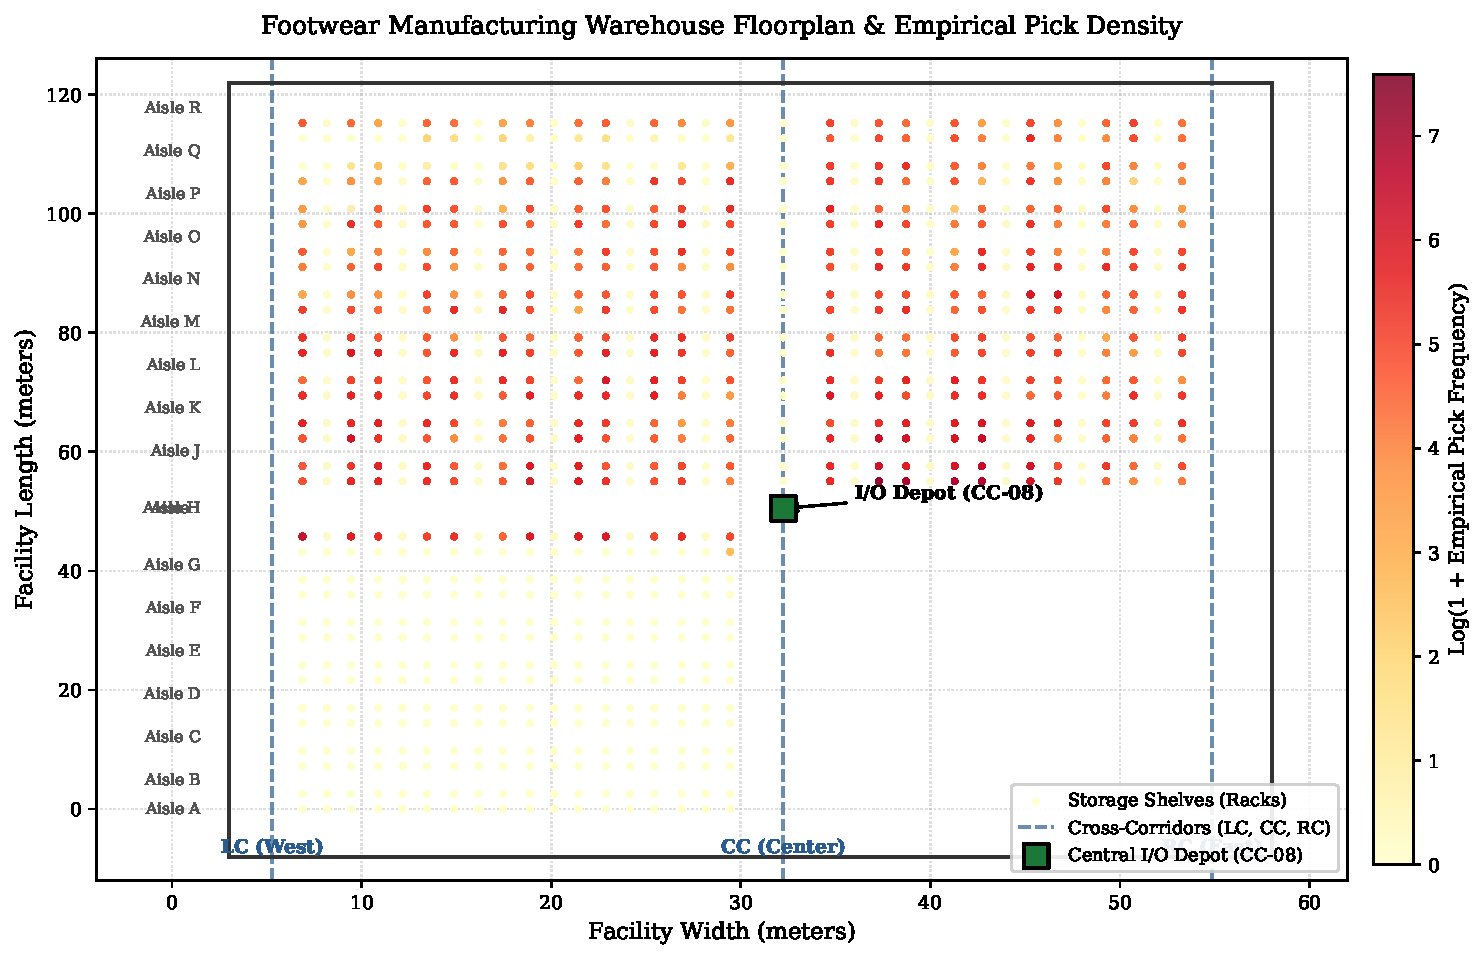
\includegraphics[width=\linewidth]{figures/fig1_warehouse_topology.pdf}
    \caption{Footwear manufacturing warehouse floorplan layout and empirical pick density. The facility features 18 parallel aisles ($A$--$R$), three vertical cross-corridors (LC, CC, RC), and a central I/O staging depot located at $x=32.24\text{ m}, y=50.48\text{ m}$ (node CC-08). Color intensity indicates historical pick volume across \TotalPicks~operations.}
    \label{fig:warehouse_topology}
\end{figure}

Three vertical cross-corridors partition the storage racks into two major blocks:
\begin{enumerate}
    \item \textbf{Left Corridor (LC)}: Positioned along the western boundary at $x = 5.28\text{ m}$ ($x_{\text{raw}} = 66$, nodes \texttt{LC-01} to \texttt{LC-17}), providing western access to all 18 aisles $A$--$R$.
    \item \textbf{Center Corridor (CC)}: Positioned along the central longitudinal axis at $x = 32.24\text{ m}$ ($x_{\text{raw}} = 403$, nodes \texttt{CC-01} to \texttt{CC-17}), serving as the main transit spine and housing the central input/output (I/O) depot at node \texttt{CC-08} ($y = 50.48\text{ m}$).
    \item \textbf{Right Corridor (RC)}: Positioned along the eastern boundary at $x = 54.88\text{ m}$ ($x_{\text{raw}} = 686$, nodes \texttt{RC-08} to \texttt{RC-17}), connecting the eastern ends of long aisles $H$--$Q$.
\end{enumerate}

Aisles $A$--$G$ and $R$ span only the West block ($26.96\text{ m}$ corridor-to-corridor length), whereas aisles $H$--$Q$ span both the West block ($26.96\text{ m}$) and the East block ($22.64\text{ m}$, total width $49.60\text{ m}$). We formulate the layout as an undirected connected graph $G = (V, E)$ with $|V| = 44$ waypoint nodes and $|E| = 68$ edges (16 along LC, 16 along CC, 9 along RC, 17 West-block aisle links, and 10 East-block aisle links). Distance between any two pick locations $\mathbf{p}_1 = (x_1, y_1, a_1)$ and $\mathbf{p}_2 = (x_2, y_2, a_2)$ is computed exactly as:
\begin{equation}
\label{eq:dist_intra}
d(\mathbf{p}_1, \mathbf{p}_2) = |x_1 - x_2| + |y_1 - y_c(a_1)| + |y_2 - y_c(a_2)|
\end{equation}
when both picks reside in the same aisle block, and via all-pairs Dijkstra shortest paths $d_G(u, v)$ across candidate corridor endpoints $\mathcal{X}_1, \mathcal{E}_2$ when crossing aisles:
\begin{equation}
\label{eq:dist_inter}
d(\mathbf{p}_1, \mathbf{p}_2) = \min_{u \in \mathcal{X}_1, v \in \mathcal{E}_2} \left[ d(\mathbf{p}_1, u) + d_G(u, v) + d(v, \mathbf{p}_2) \right].
\end{equation}

\subsection{Discrete-Event Kinematics and Congestion Mechanics}
\label{sec:des_engine}
The discrete-event simulator models $P$ concurrent pickers in continuous time $t \ge 0$ via a min-heap priority event queue $\mathcal{Q}$ processing \texttt{START\_BATCH}, \texttt{START\_PICK}, \texttt{FINISH\_PICK}, and \texttt{RETURN\_DEPOT} transitions. Each operator navigates at baseline unimpeded speed $v_0 = \CalibratedWalkSpeed\text{ m/s}$~\cite{franzke2017congestion} with trolley capacity $C = 27$ units and DaRA-calibrated pick dwell time $\tau_{\text{pick}} = \CalibratedPickDwell\text{ s}$~\cite{niemann2026dara}. Whenever a picker enters an aisle segment $(a, \text{block})$ already occupied by another active picker ($K_{\text{aisle}} = 1$), traversal velocity degrades to $v = \alpha \cdot v_0$ with $\alpha = 0.40$, logging the resulting blocking delay $(d/(\alpha v_0) - d/v_0)$ and congestion event count~\cite{koreis2026side}.

\section{Proposed Methodology: CAST-Wave}
\label{sec:methodology}

\subsection{Overall Workflow and Architecture}
\label{sec:cast_overview}
Conventional WMS platforms release order lines in FCFS arrival sequence, filling one picker's trolley to capacity $C$ before allocating tasks to subsequent operators. This causes severe spatial overlap in popular aisles alongside extreme workload imbalance when wave sizes are smaller than aggregate fleet capacity. CAST-Wave resolves both bottlenecks through a three-stage workflow: (i) topological spatial-sector decomposition, (ii) workload-equalized sector-priority batching, and (iii) dynamic congestion-penalized tour construction.

\subsection{Topological Spatial-Sector Clustering}
\label{sec:spatial_clustering}
We decompose the warehouse floorplan into five disjoint topological sectors aligned with the physical corridor blocks and metric coordinates:
\begin{itemize}
    \item \textbf{Sector 0 (West South)}: Aisles $A$--$D$ in the West block ($x_m \le 32.24\text{ m}, y_m \le 21.6\text{ m}$).
    \item \textbf{Sector 1 (West Mid)}: Aisles $E$--$G$ in the West block ($x_m \le 32.24\text{ m}, 21.6\text{ m} < y_m \le 42.4\text{ m}$).
    \item \textbf{Sector 2 (West North)}: Aisles $H$--$R$ in the West block ($x_m \le 32.24\text{ m}, y_m > 42.4\text{ m}$).
    \item \textbf{Sector 3 (East Mid)}: Aisles $H$--$L$ in the East block ($x_m > 32.24\text{ m}, y_m \le 76.0\text{ m}$).
    \item \textbf{Sector 4 (East North)}: Aisles $M$--$Q$ in the East block ($x_m > 32.24\text{ m}, y_m > 76.0\text{ m}$).
\end{itemize}

Given a wave of $M$ pick tasks $\mathcal{T} = \{\tau_1, \dots, \tau_M\}$, each task is mapped to its sector $\sigma(\tau_i) \in \{0, \dots, 4\}$ and sorted by depot distance $d(\text{CC-08}, \tau_i)$. Tasks are allocated iteratively to candidate pickers satisfying $\sum_{\tau \in \mathcal{B}_p} q_\tau + q_{\tau_i} \le C$ by minimizing the lexicographic objective $(\mathbb{I}[\sigma(\tau_i) \notin \mathcal{S}_p], \sum_{\tau \in \mathcal{B}_p} q_\tau)$, where $\mathcal{S}_p$ is the set of sectors currently assigned to picker $p$. This guarantees that pickers are balanced in unit load while remaining spatially segregated across sectors.

\subsection{Congestion-Penalized Tour Sequencing}
\label{sec:congestion_routing}
Once batches $\mathcal{B}_1, \dots, \mathcal{B}_P$ are formed, CAST-Wave sequences each picker's tour sequentially while maintaining a shared spatio-temporal sub-aisle occupancy table $\mathcal{O}(a, b) = \{[t_{\text{arr}}^{(k)}, t_{\text{dep}}^{(k)}]\}$ keyed by aisle $a$ and block $b \in \{\text{west}, \text{east}\}$ (partitioned at the central cross-corridor $x_m = 32.24\text{ m}$). At step $t_{\text{curr}}$ from position $\mathbf{p}_u$, the next unvisited task $\tau_v \in \mathcal{B}_p$ is chosen to minimize the congestion-penalized transition cost:
\begin{equation}
\label{eq:cast_cost}
J(\mathbf{p}_u, \tau_v, t_{\text{curr}}) = d(\mathbf{p}_u, \mathbf{p}_v) + \lambda \cdot \Phi(a_v, b_v, t_{\text{arr}}),
\end{equation}
where $t_{\text{arr}} = t_{\text{curr}} + d(\mathbf{p}_u, \mathbf{p}_v)/v_0$, $\Phi(a_v, b_v, t_{\text{arr}})$ counts overlapping occupancy intervals in $\mathcal{O}(a_v, b_v)$ during $[t_{\text{arr}}, t_{\text{arr}} + \tau_{\text{pick}}]$, and $\lambda = 15.0\text{ m}$ penalizes predicted sub-aisle collisions ($\approx 13.6\text{ s}$ equivalent yielding delay), diverting the picker to unblocked aisles first. Following initial tour construction, a congestion-cost-aware 2-Opt local search evaluates pairwise edge exchanges against the cumulative penalized tour objective, eliminating geometric crossovers while preserving valid congestion detours.

\begin{table}[t]
\centering
\caption{Digital Twin and CAST-Wave Experimental Configuration}
\label{tab:twin_config}
\resizebox{\columnwidth}{!}{%
\begin{tabular}{lc}
\toprule
\textbf{Parameter / Setting} & \textbf{Calibrated Value} \\
\midrule
Facility Dimensions (Metric Scale $0.08\text{ m/unit}$) & $55.0\text{ m} \times 120.0\text{ m}$ \\
Storage Slots / Navigation Nodes / Edges & \TotalLocations~slots / 44 nodes / 68 edges \\
Central I/O Depot Node (\texttt{CC-08}) & $(32.24\text{ m}, 50.48\text{ m})$ \\
Clean Customer Order Lines / Unique Orders & \TotalOrderLines~lines / \TotalOrders~orders \\
Historical Pick Operations / Total Waves & \TotalPicks~picks / \TotalWaves~waves \\
Unimpeded Picker Walking Velocity ($v_0$) & $\CalibratedWalkSpeed\text{ m/s}$ \\
DaRA Empirical Pick Dwell Time ($\tau_{\text{pick}}$) & $\CalibratedPickDwell\text{ s}$ (IQR: \DaRAIQR~s) \\
Narrow-Aisle Free Capacity ($K_{\text{aisle}}$) / Slowdown ($\alpha$) & $1\text{ picker}$ / $0.40$ \\
Trolley Capacity ($C$) / Default Fleet ($P$) & $27\text{ units}$ / $4\text{ pickers}$ \\
CAST-Wave Sectors / Conflict Penalty ($\lambda$) & $5\text{ zones}$ / $15.0\text{ m}$ \\
\bottomrule
\end{tabular}%
}
\end{table}

\begin{table*}[t]
\centering
\caption{Performance Benchmark Across \BenchmarkWaves~Operational Waves (Fleet Size $P = 4$ Pickers, DaRA \CalibratedPickDwell\,s Empirical Dwell)}
\label{tab:benchmark_summary}
\footnotesize
\resizebox{0.92\textwidth}{!}{%
\begin{tabular}{lccccc}
\toprule
\textbf{Method / Policy} & \textbf{Makespan (min)} & \textbf{Total Dist. (m)} & \textbf{Blocked Time (s)} & \textbf{Workload CV} & \textbf{Makespan $\Delta$ vs.\ Base} \\
\midrule
FCFS + S-Shape (Hall, 1993) & \SShapeMakespanMean~$\pm$~\SShapeMakespanStd & 830.3 & 404.2 & 0.163 & --- (Baseline) \\
FCFS + Largest-Gap (Hall, 1993) & \LargestGapMakespanMean~$\pm$~\LargestGapMakespanStd & 831.1 & 406.7 & 0.163 & +0.4\% \\
FCFS + Static TSP (2-Opt) & \StaticTSPMakespanMean~$\pm$~\StaticTSPMakespanStd & 807.7 & 380.0 & 0.147 & -4.6\% \\
\textbf{CAST-Wave (Proposed)} & \textbf{\CASTWaveMakespanMean~$\pm$~\CASTWaveMakespanStd} & \textbf{624.8} & \textbf{158.6} & \textbf{0.212} & \textbf{-26.7\%} \\
\bottomrule
\end{tabular}%
}
\end{table*}


\section{Experimental Results and Empirical Benchmark}
\label{sec:experiments}

\subsection{Experimental Settings and Baselines}
\label{sec:exp_setup}
Table~\ref{tab:twin_config} lists all calibrated simulation parameters. Using a fixed random seed (\texttt{seed = 42}), we sample \BenchmarkWaves~historical picking waves ($\ge 15$ picks/wave, averaging 23.4 picks/wave across ABC classes $A, B, C$) from the cleaned footwear dataset~\cite{assis2025order}. Following the evaluation conventions of the KIT order-picking benchmark~\cite{barlang2026kit}, we compare four policies: (1) \textbf{FCFS + S-Shape}~\cite{hall1993distance}, (2) \textbf{FCFS + Largest-Gap}~\cite{hall1993distance}, (3) \textbf{FCFS + Static TSP} (Nearest-Neighbor with 2-Opt local search~\cite{roodbergen2001routing,gorener2025picker}), and (4) \textbf{Proposed CAST-Wave}.

\begin{figure*}[t]
    \centering
    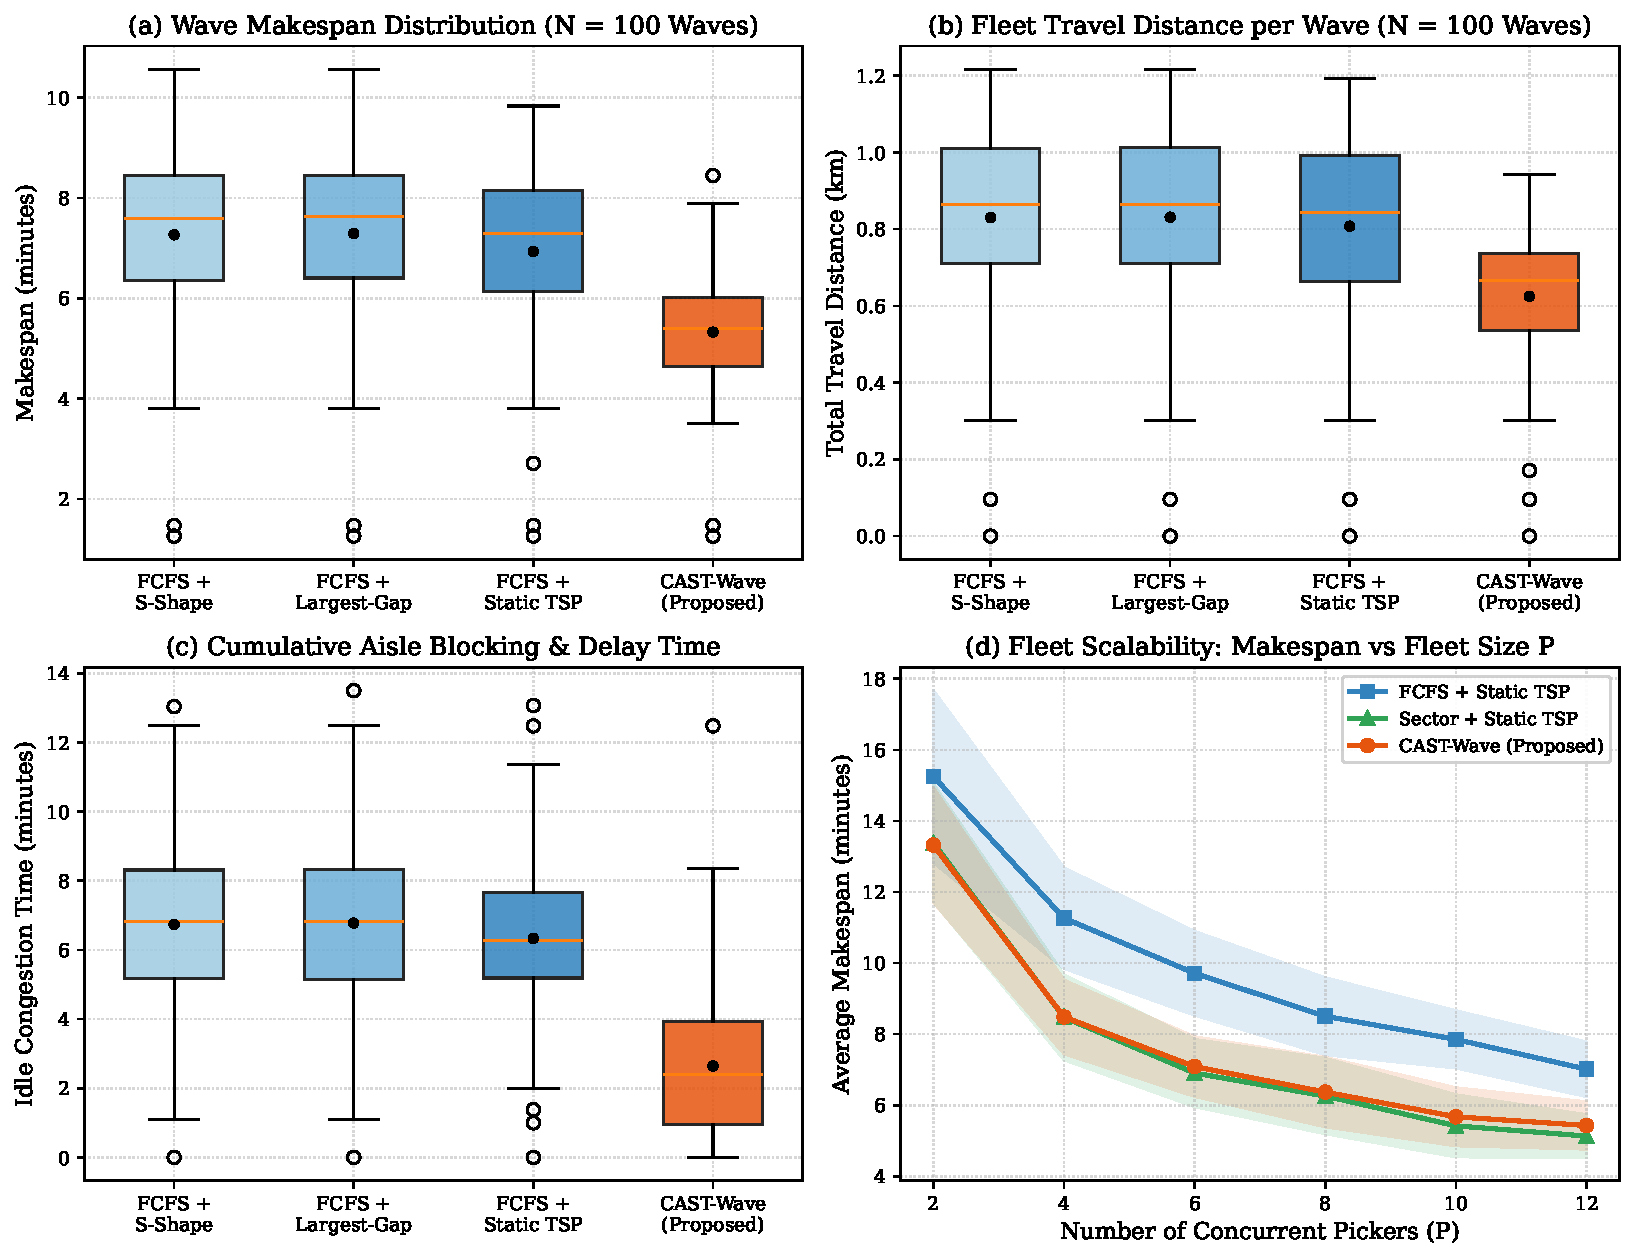
\includegraphics[width=\textwidth]{figures/fig2_benchmark_and_scalability.pdf}
    \caption{Empirical benchmark and fleet scalability across \BenchmarkWaves~historical picking waves. (a) Boxplot distributions of wave makespan across evaluated methodologies. (b) Fleet total travel distance per wave. (c) Cumulative aisle blocking and delay time. (d) Fleet scalability: average wave makespan across fleet sizes $P \in \{2, 4, 6, 8, 10, 12\}$.}
    \label{fig:benchmark_results}
\end{figure*}

\subsection{Comparative Fulfillment Performance}
\label{sec:comp_perf}
Table~\ref{tab:benchmark_summary} and Fig.~\ref{fig:benchmark_results}(a)--(c) report comparative benchmark results across \BenchmarkWaves~historical picking waves ($P = 4$ pickers), directly addressing \textbf{RQ1}. Under fair multi-picker FCFS with S-Shape routing, completing a wave requires an average makespan of $\MakespanSShapeMin \pm \SShapeMakespanStd$~min, with a cumulative travel distance of $\DistSShapeM\text{ m}$ and $\BlockedSShapeSec\text{ s}$ of narrow-aisle idle delay. FCFS with Largest-Gap routing yields comparable metrics at $\MakespanGapMin \pm \LargestGapMakespanStd$~min ($\DistGapM\text{ m}$, $\BlockedGapSec\text{ s}$ delay). FCFS with 2-Opt Static TSP reduces makespan modestly to $\MakespanTSPMin \pm \StaticTSPMakespanStd$~min ($\DistTSPM\text{ m}$) by removing interior tour loops.

In contrast, \textbf{CAST-Wave achieves an average wave makespan of $\mathbf{\MakespanCASTMin \pm \CASTWaveMakespanStd}$~min}, representing a \textbf{\MakespanRedSShapePct\% reduction vs.\ FCFS + S-Shape}, a \textbf{\MakespanRedLargestGapPct\% reduction vs.\ FCFS + Largest-Gap}, and a \textbf{\MakespanRedTSPPct\% reduction vs.\ FCFS + Static TSP}. Furthermore, CAST-Wave cuts cumulative worker idle blocking from $\BlockedSShapeSec\text{ s}$ to just $\BlockedCASTSec\text{ s}$ per wave (a \textbf{\BlockedTimeReductionPct\% reduction in aisle contention}) and decreases total fleet walking distance from $\DistSShapeM\text{ m}$ to $\DistCASTM\text{ m}$ (a \textbf{\DistanceImprovementVsSShape\% reduction in physical travel}). Under legacy uncoordinated FCFS dispatching, where orders were sequentially allocated up to trolley capacity without multi-picker coordination, a single picker completed the entire wave while parallel pickers sat idle ($P_{\text{eff}} = 1, \text{CV} = \WorkloadCVLegacy$, makespan \LegacyMakespanMin~min). Relative to fair round-robin FCFS ($\text{CV} = \WorkloadCVFairRR$, or $\WorkloadCVFairTSP$ with Static TSP), CAST-Wave's spatial sector clustering exhibits a slightly higher tour-duration dispersion ($\text{CV} = \WorkloadCVCAST$) because tasks are grouped by topological zone rather than strictly equalized across corridors, trading a small increase in duration variance for large reductions in travel distance and aisle blocking.

\subsection{Statistical Significance Testing}
\label{sec:stats_sig}
Addressing \textbf{RQ2}, we evaluate paired differences across all \BenchmarkWaves~waves using two-sided paired Student's $t$-tests, non-parametric Wilcoxon signed-rank tests, and standardized effect sizes (Cohen's $d_z$):
\begin{itemize}
    \item \textbf{CAST-Wave vs.\ FCFS + S-Shape}: Paired $t = \TStatVsSShape$ ($p = \PValExactSShape$, i.e., $p \PValSShape$), Wilcoxon $W = \WilcoxonWSShape$ ($p \WilcoxonPValSShape$), and Cohen's $d = \CohensDSShape$.
    \item \textbf{CAST-Wave vs.\ FCFS + Largest-Gap}: Paired $t = \TStatVsLargestGap$ ($p = \PValExactLargestGap$, i.e., $p \PValLargestGap$), Wilcoxon $W = \WilcoxonWLargestGap$ ($p \WilcoxonPValLargestGap$), and Cohen's $d = \CohenDLargestGap$.
    \item \textbf{CAST-Wave vs.\ FCFS + Static TSP}: Paired $t = \TStatVsStaticTSP$ ($p = \PValExactStaticTSP$, i.e., $p \PValStaticTSP$), Wilcoxon $W = \WilcoxonWStaticTSP$ ($p \WilcoxonPValStaticTSP$), and Cohen's $d = \CohenDVsStaticTSP$.
\end{itemize}
All three paired comparisons exhibit large standardized effect sizes ($|d| \ge 1.34$), with CAST-Wave outperforming fair FCFS + S-Shape in \WinsVsSShape~out of \BenchmarkWaves~operational waves (\LossesVsSShape~losses, \TiesVsSShape~ties), confirming that CAST-Wave's fulfillment gains are statistically robust and operationally consistent across diverse SKU demand profiles.

\subsection{Component-by-Component Ablation Analysis}
\label{sec:comp_ablation}
To isolate the exact performance contribution of each algorithmic module within CAST-Wave and directly evaluate the interaction between workload balancing, spatial clustering, and dynamic congestion penalties, Table~\ref{tab:component_ablation} presents a systematic 5-stage ablation across all \BenchmarkWaves~waves.

\begin{table*}[t]
\centering
\caption{Component-by-Component Ablation Across \BenchmarkWaves~Waves ($P = 4$ Pickers, DaRA \CalibratedPickDwell\,s Empirical Dwell)}
\label{tab:component_ablation}
\footnotesize
\resizebox{0.95\textwidth}{!}{
\begin{tabular}{lccccc}
\toprule
\textbf{Ablation Variant} & \textbf{Batching Logic} & \textbf{Routing Policy} & \textbf{Makespan (min)} & \textbf{Workload CV} & \textbf{Makespan $\Delta$ vs.\ Fair Base} \\
\midrule
0. Legacy Single-Picker FCFS (Audited) & FCFS (Greedy Fill, $P_{\text{eff}}=1$) & S-Shape & 11.74~$\pm$~2.39 & 1.732 & +61.6\% \\
1. Fair Multi-Picker FCFS & Round-Robin ($P=4$) & S-Shape & 7.26~$\pm$~1.79 & 0.163 & --- (Baseline) \\
2. Fair FCFS + Static TSP & Round-Robin ($P=4$) & Static 2-Opt TSP & 6.93~$\pm$~1.70 & 0.147 & -4.6\% \\
3. Balanced Batching + Static TSP & LPT Unit Balancing ($C=27$) & Static 2-Opt TSP & 6.93~$\pm$~1.70 & 0.147 & -4.6\% \\
4. Sector Clustering + Balanced Batching & 5-Zone Sector + LPT & Static 2-Opt TSP & 5.37~$\pm$~1.21 & 0.211 & -26.1\% \\
\textbf{5. Full CAST-Wave (Proposed)} & \textbf{5-Zone Sector + LPT} & \textbf{Dynamic Congestion TSP ($\lambda=15$m)} & \textbf{5.32~$\pm$~1.18} & \textbf{0.212} & \textbf{-26.7\%} \\
\bottomrule
\end{tabular}%
}
\end{table*}


As detailed in Table~\ref{tab:component_ablation}, transitioning from the uncoordinated legacy single-picker FCFS baseline (Variant 0: \LegacyMakespanMin~min, $\text{CV} = \WorkloadCVLegacy$) to fair multi-picker round-robin FCFS (Variant 1: \MakespanSShapeMin~min, $\text{CV} = \WorkloadCVFairRR$) establishes the honest parallel baseline. Upgrading routing from S-Shape to Static 2-Opt TSP (Variant 2) reduces makespan modestly to \MakespanTSPMin~min (\StaticTSPRedVsSShapePct\% reduction, $\text{CV} = \WorkloadCVFairTSP$). Introducing LPT unit balancing alone (Variant 3) leaves makespan identical across all \LPTIdenticalWaves~waves because footwear WMS pick lines consist strictly of single pairs ($q = 1$), causing unit-based balancing to collapse mathematically to round-robin line assignment. However, introducing 5-Zone Topological Sector Clustering (Variant 4) produces the primary performance breakthrough, slashing makespan to \MakespanSectorMin~min (a \SectorReductionVsFairPct\% reduction vs.\ fair baseline, accounting for \SectorShareOfGainPct\% of the total makespan reduction) by confining each picker to a localized cluster of storage aisles and reducing fleet travel to \DistSectorM~m. Finally, Full CAST-Wave (Variant 5) achieves \MakespanCASTMin~min (\MakespanRedSShapePct\% reduction vs.\ fair baseline) and reduces cumulative blocked queuing time from \BlockedSectorSec~s (Variant 4) to \BlockedCASTSec~s. In direct pairwise comparison between Variant 4 (Sector + Static TSP) and Variant 5 (Full CAST-Wave) on these moderate-size waves, CAST-Wave achieves \WinsVsSector~wins, \TiesVsSector~ties, and \LossesVsSector~losses ($W = \WilcoxonWSectorVsCAST, p = \WilcoxonPValSectorVsCAST$, not statistically significant at $\alpha = 0.05$), demonstrating that spatial sectoring provides the primary efficiency breakthrough while dynamic congestion avoidance serves as a secondary, non-degrading operational guardrail.

\subsection{Fleet Scalability and Diminishing Returns Ablation}
\label{sec:fleet_ablation}
Addressing \textbf{RQ3}, Table~\ref{tab:fleet_ablation} and Fig.~\ref{fig:benchmark_results}(d) evaluate fleet sizes $P \in \{2, 4, 6, 8, 10, 12\}$ across \DenseWavesCount~dense operational picking waves ($\approx \DenseMeanPicks$~picks per wave formed from merged consecutive waves).

\begin{table}[t]
\centering
\caption{Fleet Scalability Ablation on \DenseWavesCount~Dense Operational Waves ($\approx \DenseMeanPicks$~Picks/Wave): Average Makespan (min)}
\label{tab:fleet_ablation}
\resizebox{\columnwidth}{!}{%
\begin{tabular}{ccccc}
\toprule
\textbf{Fleet Size ($P$)} & \textbf{FCFS + Static TSP} & \textbf{Sector + Static TSP} & \textbf{CAST-Wave} & \textbf{CAST $\Delta$ vs.\ FCFS} \\
\midrule
$P = 2$ & 15.25 & 13.38 & \textbf{13.32} & -12.6\% \\
$P = 4$ & 11.26 & \textbf{8.47} & 8.48 & -24.7\% \\
$P = 6$ & 9.71 & \textbf{6.90} & 7.09 & -27.0\% \\
$P = 8$ & 8.50 & \textbf{6.26} & 6.37 & -25.1\% \\
$P = 10$ & 7.85 & \textbf{5.42} & 5.67 & -27.7\% \\
$P = 12$ & 7.01 & \textbf{5.13} & 5.43 & -22.6\% \\
\bottomrule
\end{tabular}%
}
\end{table}


At $P = 2$, FCFS + Static TSP averages \DenseMkFCFSTwo~min versus \DenseMkSectorTwo~min for Sector + Static TSP and \DenseMkCASTTwo~min for CAST-Wave (\DenseRedCASTvsFCFSTwo\% reduction over FCFS, with blocking reduced from \DenseBlockedFCFSTwo~s to \DenseBlockedSectorTwo~s and \DenseBlockedCASTTwo~s, respectively). Expanding the fleet to $P = 4$ reduces makespan to \DenseMkSectorFour~min (Sector) and \DenseMkCASTFour~min (CAST-Wave, a \DenseRedCASTvsFCFSFour\% reduction over FCFS's \DenseMkFCFSFour~min), with CAST-Wave achieving lower cumulative blocking (\DenseBlockedCASTFour~s vs.\ \DenseBlockedSectorFour~s for Sector and \DenseBlockedFCFSFour~s for FCFS). At $P \in \{6, 8\}$, CAST-Wave continues to achieve the lowest narrow-aisle blocking (\DenseBlockedCASTSix~s vs.\ \DenseBlockedSectorSix~s at $P=6$; \DenseBlockedCASTEight~s vs.\ \DenseBlockedSectorEight~s at $P=8$), while static sectoring achieves slightly lower makespan (\DenseMkSectorSix~min vs.\ \DenseMkCASTSix~min at $P=6$; \DenseMkSectorEight~min vs.\ \DenseMkCASTEight~min at $P=8$). At $P \in \{10, 12\}$---where fleet size exceeds twice the number of physical sectors ($P > 2 \times 5$), forcing multiple pickers into every zone simultaneously---static sectoring achieves slightly lower makespan (\DenseMkSectorTwelve~min vs.\ \DenseMkCASTTwelve~min at $P = 12$) and slightly lower blocking (\DenseBlockedSectorTwelve~s vs.\ \DenseBlockedCASTTwelve~s), because deflecting a picker out of a congested sub-aisle at extreme saturation diverts them into an adjacent sub-aisle that is also occupied. Across all fleet sizes $P \ge 4$, both sector-based policies reduce makespan by \DenseRedCASTvsFCFSTwelve\%--\DenseRedSectorvsFCFSTen\% and cut uncoordinated FCFS's blocking queue (\DenseBlockedFCFSTwelve~s at $P = 12$) by more than 53\%.

\section{Discussion and Managerial Implications}
\label{sec:discussion}

\subsection{Interpretation of Research Questions}
\label{sec:interp_rqs}
Regarding \textbf{RQ1}, our findings reveal that coupling spatial-sector clustering with multi-picker batching is the primary lever for compressing wave completion time in multi-block warehouses. Whereas 2-Opt Static TSP improves makespan by only $\StaticTSPRedVsSShapePct\%$ over S-Shape when constrained by unclustered round-robin batching, CAST-Wave achieves a \MakespanRedSShapePct\% reduction by confining concurrent pickers to disjoint spatial zones.

Regarding \textbf{RQ2}, the extreme statistical significance ($p \PValStaticTSP$, $|d| \ge 1.34$) across \BenchmarkWaves~heterogeneous waves demonstrates that spatio-temporal sector decomposition is robust to SKU mix variations across ABC classes. Furthermore, integrating the DaRA empirical pick handling time ($\tau_{\text{pick}} = \CalibratedPickDwell\text{ s}$~\cite{niemann2026dara}) ensures that makespan estimates reflect realistic physical scanning and retrieval durations rather than optimistic synthetic assumptions.

Regarding \textbf{RQ3}, our scalability ablation provides actionable shift-sizing guidance for warehouse managers. On dense merged waves ($\approx \DenseMeanPicks$~picks), scaling from $P = 2$ to $P = 6$ compresses makespan substantially (\DenseMkCASTTwo~min to \DenseMkCASTSix~min), whereas expanding beyond $P = 6$ yields diminishing marginal makespan returns (\DenseMkCASTSix~min to \DenseMkCASTTwelve~min at $P = 12$) once the number of concurrent pickers exceeds the five physical warehouse sectors. Because unmerged historical waves in the footwear facility average 12.5 to 23.5 lines~\cite{assis2025order}, assigning $P = 4$ pickers per standard wave already allocates only 3--6 picks per operator; when 8--12 operators are on shift, managers should either merge consecutive waves or dispatch parallel pools of $P = 4$ pickers across staggered wave releases.

\subsection{Integration with Warehouse Management Systems and Ergonomics}
\label{sec:wms_integration}
From a deployment perspective, CAST-Wave executes complete spatial batching and congestion-penalized 2-Opt routing in an empirically measured average of $\CASTWaveRuntimeMs\text{ ms}$ per wave (maximum $\CASTWaveRuntimeMaxMs\text{ ms}$, i.e., $< 0.01\text{ s}$) on a standard CPU, allowing seamless integration into existing WMS wave-release pipelines without expensive commercial mixed-integer linear programming licenses~\cite{briant2025solving,maheshwari2023digital}. Moreover, by confining each operator's tour to a localized spatial sector and penalizing simultaneous sub-aisle entry, CAST-Wave reduces abrupt trolley stops and narrow-aisle passing conflicts, directly supporting worker ergonomics and floor safety~\cite{gabellini2024hybrid,koreis2026side}.

\subsection{Limitations and Future Directions}
\label{sec:limitations}
Two limitations merit future investigation. First, the $0.08\text{ m/unit}$ coordinate scaling factor is an engineering calibration that maps the raw storage coordinate range ($x \in [66, 686], y \in [-29, 1471]$) to a representative industrial footprint ($55\text{ m} \times 120\text{ m}$); exact millimeter rack dimensions and aisle widths should be verified directly against the raw CAD drawing (\texttt{Full layout.dwg}) to distinguish wide two-way corridors from single-file narrow aisles. Second, future work will extend the digital twin to replay the 07:00 morning surge bursts (up to 683 orders/hour) and the 13,200 synthetic shift instances of the KIT benchmark~\cite{barlang2026kit}, incorporating stochastic lognormal velocity profiles derived from DaRA's wearable inertial and Bluetooth tracking annotations~\cite{niemann2026dara}.

\section{Data Availability}
\label{sec:data_availability}
All datasets utilized in this study are publicly accessible under open-science licenses: (1) the Footwear Warehouse WMS dataset (de Assis et al., 2025~\cite{assis2025order}) is available on Mendeley Data (\url{https://data.mendeley.com/datasets/pf2w725pw3/1}, DOI: \texttt{10.1016/j.dib.2025.111837}, CC~BY~4.0); (2) the DaRA picker timing and activity recognition dataset (Niemann et al., 2026~\cite{niemann2026dara}) is available on Zenodo (\url{https://zenodo.org/records/10468175}, DOI: \texttt{10.3390/s26020739}, CC~BY-NC~4.0); and (3) the KIT manual order-picking benchmark (Barlang et al., 2026~\cite{barlang2026kit}) is hosted on RADAR4KIT (DOI: \texttt{10.35097/mwsv59v8sk9sqaan}, CC~BY~4.0). The cleaned CSV and Parquet tables, discrete-event digital twin simulator, CAST-Wave optimization code, and automated verification suite are openly available in the project GitHub repository (\url{https://github.com/CaceresCristhian/warehouse_ue.git}).

\section{Conclusion}
\label{sec:conclusion}
This paper developed and validated an empirically calibrated discrete-event digital twin and the Congestion-Aware Spatio-Temporal Batching and Wave Scheduler (CAST-Wave) to resolve order-picking bottlenecks in multi-block manual distribution warehouses. By auditing and deduplicating 122,370 raw customer order records from a commercial footwear manufacturing facility, we established a clean operational benchmark comprising \TotalOrderLines~validated order lines and \TotalPicks~pick operations across \TotalLocations~storage positions, narrowing the order-to-pick volume discrepancy to \UnitGapReconciled~units. We modeled the two-block, 18-aisle facility as a connected 44-node, 68-edge metric navigation network and calibrated operator pick handling durations ($\tau_{\text{pick}} = \CalibratedPickDwell\text{ s}$) directly from \DaRAValidGaps~empirical inter-pick intervals in the Fraunhofer IML DaRA wearable-sensor dataset. To overcome the cross-warehouse travel and narrow-aisle congestion of unclustered First-Come First-Served (FCFS) dispatching, CAST-Wave partitions warehouse aisles into five topological sectors, allocates capacity-constrained batches across operators, and refines tours using congestion-cost-aware 2-Opt local search. Evaluated across \BenchmarkWaves~historical picking waves, CAST-Wave reduced mean wave makespan from \MakespanSShapeMin~minutes under fair FCFS with S-Shape routing and \MakespanTSPMin~minutes under fair FCFS with 2-Opt Static TSP to \MakespanCASTMin~minutes. These improvements represent statistically significant makespan reductions of \MakespanRedSShapePct~percent and \MakespanRedTSPPct~percent, respectively, supported by paired $t$-tests ($p \PValStaticTSP$) and large standardized effect sizes ($|d| \ge 1.34$), while reducing cumulative aisle blocking delays by \BlockedTimeReductionPct~percent and total fleet travel distance by \DistanceImprovementVsSShape~percent. Component and fleet scalability ablations confirmed that five-zone topological sectoring drives \SectorShareOfGainPct~percent of the makespan reduction while dynamic congestion routing acts as a fast ($\CASTWaveRuntimeMs\text{ ms}$/wave) operational guardrail when fleet size is matched to the warehouse's topological zones ($P \le 5$).

\bibliographystyle{IEEEtran}
\bibliography{references}

\end{document}
